\documentclass{article}
\usepackage[utf8]{inputenc}
\usepackage{graphicx}
\graphicspath{ {./images/} }

\begin{document}
\title{UNIBOssfight}
\author{Livia Cardaccia, Denise Nanni, Giovanni Prete, Matteo Sartini}
\date{January 2023}
\maketitle
\newpage
\large
\tableofcontents
\newpage

\section{Analisi}

\subsection{Requisiti} 
Il team si pone come obiettivo quello di realizzare una versione personalizzata del noto gioco arcade Metal Slug, ambientato nella nostra università. 
Lo scopo del gioco è quello di conseguire la laurea superando gli esami, rappresentati da una serie di livelli platform, ossia in cui la meccanica di gioco implica principalmente l'attraversamento di livelli costituiti da piattaforme, spesso disposte su più piani.
In ogni livello sono presenti diversi minions che ostacolano la corsa del giocatore, e un boss finale, rappresentato dal docente del corso, la cui sconfitta determinerà il superamento dell'esame. 
\subsubsection{Requisiti funzionali}
\begin{itemize}
    \item Menù principale che permette all'utente di scegliere il livello di gioco, consultare i comandi, iniziare una nuova partita e uscire dal gioco.
    \item Gestione dell'input simultaneo per il movimento e la gestione dell'arma.
    \item Movimento di base dei nemici.
    \item Implementazione di un'arma a fuoco automatico che verrà puntata in base alla posizione del mouse.
    \item Calcolo del voto finale basato nemici sconfitti
    e monete CFU raccolte.
\end{itemize}
\subsubsection{Requisiti non funzionali}
\begin{itemize}
    \item Il gioco dovrà risultare fluido, con un frame rate minimo di 30 FPS.
    \item Il gioco avrà una bassa latenza di input
\end{itemize}
\subsection{Analisi e modello del dominio}
Il giocatore dovrà superare una serie di livelli in cui incontrerà due tipologie di ostacoli: nemici in movimento, che possono provocargli danno, e ostacoli di tipo ambientale.
Il giocatore potrà affrontare i nemici con l'arma in dotazione, stando attento a non esaurire la vita a sua disposizione, o scegliere di evitarli quando possibile (pena decurtazione del punteggio).
Gli ostacoli ambientali invece consisteranno in muri da scavalcare, fiamme e spine da evitare.
Alla fine del livello il personaggio si troverà ad affrontare un boss finale che disporrà di una quantità superiore di punti vita e arrecherà più danno rispetto ai nemici comuni.


\section{Design}
\subsection{Architettura}
Questo progetto è stato sviluppato attraverso il pattern architetturale ECS, Entity Component System.
In ECS, le Entity sono tutte le entità di gioco, ovvero degli oggetti general purpose, che si compongono dei Components; questi ultimi modellano una determinata caratteristica di un'entità e mantengono i dati relativi ad essa. Il System è tutto ciò che modifica le entità, agendo sui loro componenti. Nella nostra applicazione le entity sono tutti gli attori del mondo di gioco, ad esempio il giocatore e i nemici, decorati da componenti che modellano il concetto di movimento e posizione con il \texttt{Transform}, le collisioni con il \texttt{Collider}, il comportamento con il \texttt{Behaviour} e simili, i quali vengono gestiti dal \texttt{Level} che rappresenta il sistema.
Nonostante non avessimo affrontato a lezione il pattern ECS, lo abbiamo scelto perché ci sembrava adatto ad un progetto come il nostro, dato che viene ampiamente utilizzato nello sviluppo di videogiochi, è versatile e facilmente estendibile.
L'aspetto caratteristico di ECS è che ogni entità si autogestisce, sia per quanto riguarda aspetti come il movimento, sia per altri aspetti come la renderizzazione; per tale motivo, utilizzando questo pattern potrebbe risultare poco agevole sostituire in blocco la view, tuttavia può essere fatto effettuando delle modifiche minori, in particolare al component \texttt{Renderer}.



\subsection{Design dettagliato}
\subsubsection{Livia Cardaccia}

\subsubsection{Denise Nanni}
bla bla bla
\begin{figure}[ht]
    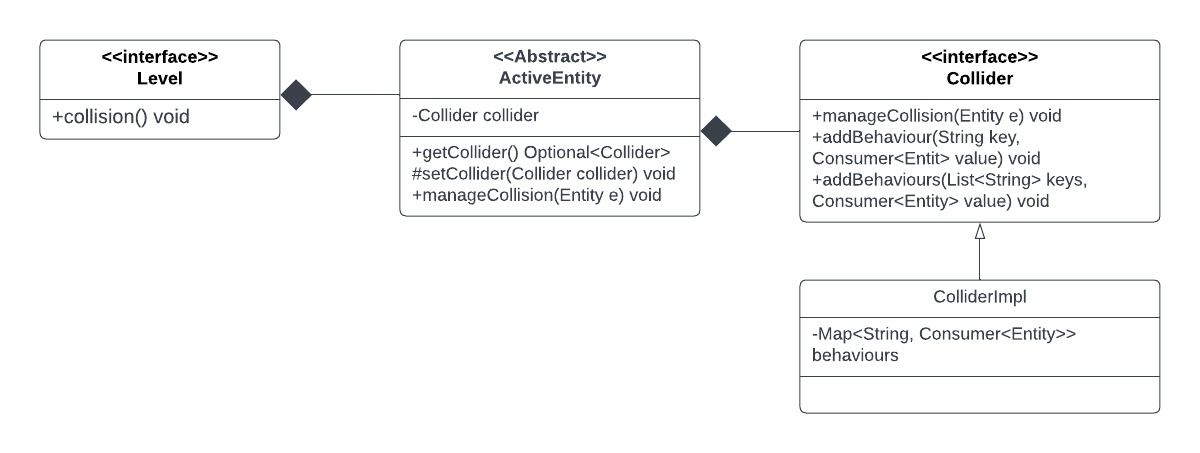
\includegraphics[width=1\textwidth]{umlCollider.jpg}
    \caption{descrizione}
    \label{fig:schgen}
\end{figure}
\subsubsection{Giovanni Prete}
\subsubsection{Matteo Sartini}
Il mio task principale all’interno del progetto consisteva nell’implementare un sistema che permettesse alle entità di sparare all’interno del livello in cui agiscono.
Per fare ciò in fase di progettazione, in linea con il modello ECS, abbiamo deciso di implementare un component Weapon, che permettesse alle entità che ne erano in possesso di creare nuove entità Bullet e dare loro una traiettoria verso cui muoversi.
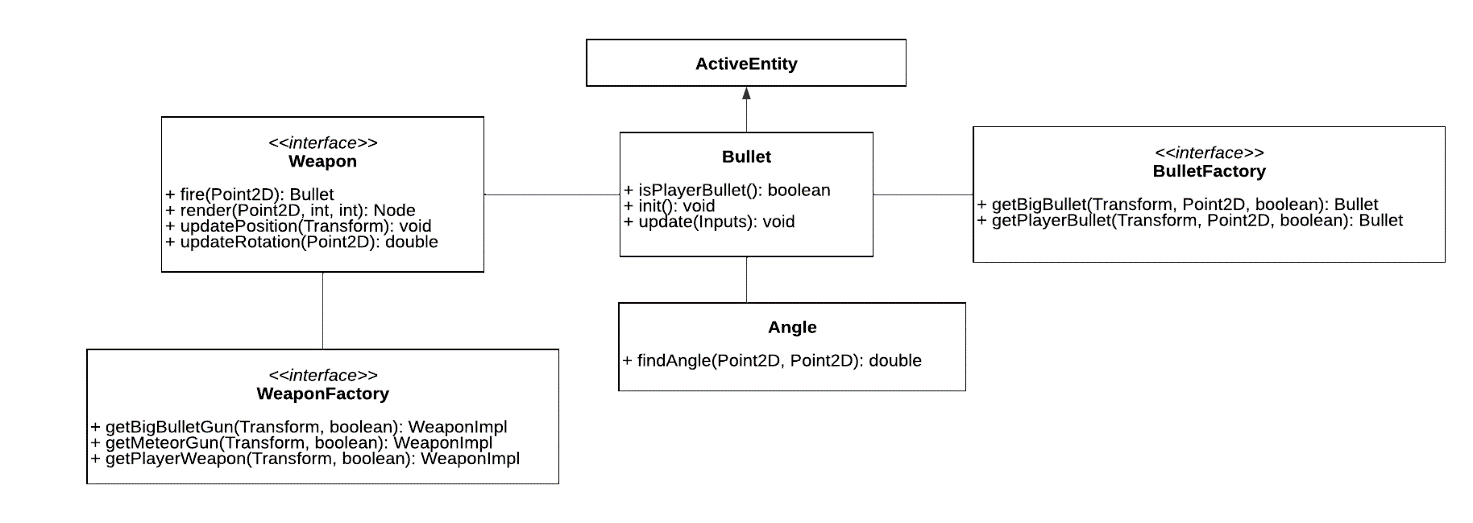
\includegraphics[width=1\textwidth]{UMLWeapon.png}
    \caption{UML rappresentante Weapon e Bullet}
    \label{fig:schgen}
Richiamando il metodo fire viene restituita una nuova istanza dell’entità Bullet, creata attraverso l’utilizzo di una apposita Factory. A questa Entità Bullet vengono passate delle coordinate che rappresentano il punto mirato dalla entità (nel caso del player queste sono le coordinate del puntatore del mouse) che utilizza per estrapolare la traiettoria da mantenere per colpire il punto desiderato. Per fare questo ho ritenuto necessaria la scrittura di una classe utility Angle che mi permettesse di trovare l’angolo formato dal vettore teso tra due punti noti e il piano di riferimento del sistema. Il bullet una volta generato sarà gestito insieme alle altre entity del livello.
La classe Angle citata in precedenza è inoltre utilizzata per gestire la rotazione dell’arma del Player che è sempre orientata verso il puntatore del mouse.
Weapon oltre alla sua funzione principale permette anche di essere renderizzato in sovrapposizione al suo user tramite un component Renderer. La posizione di renderizzazione dell’arma e la posizione da cui vengono sparati i Bullet vengono aggiornate tramite un proprio component Transform durante l’update dell’entity a cui appartengono in base alla posizione di quest’ultima.
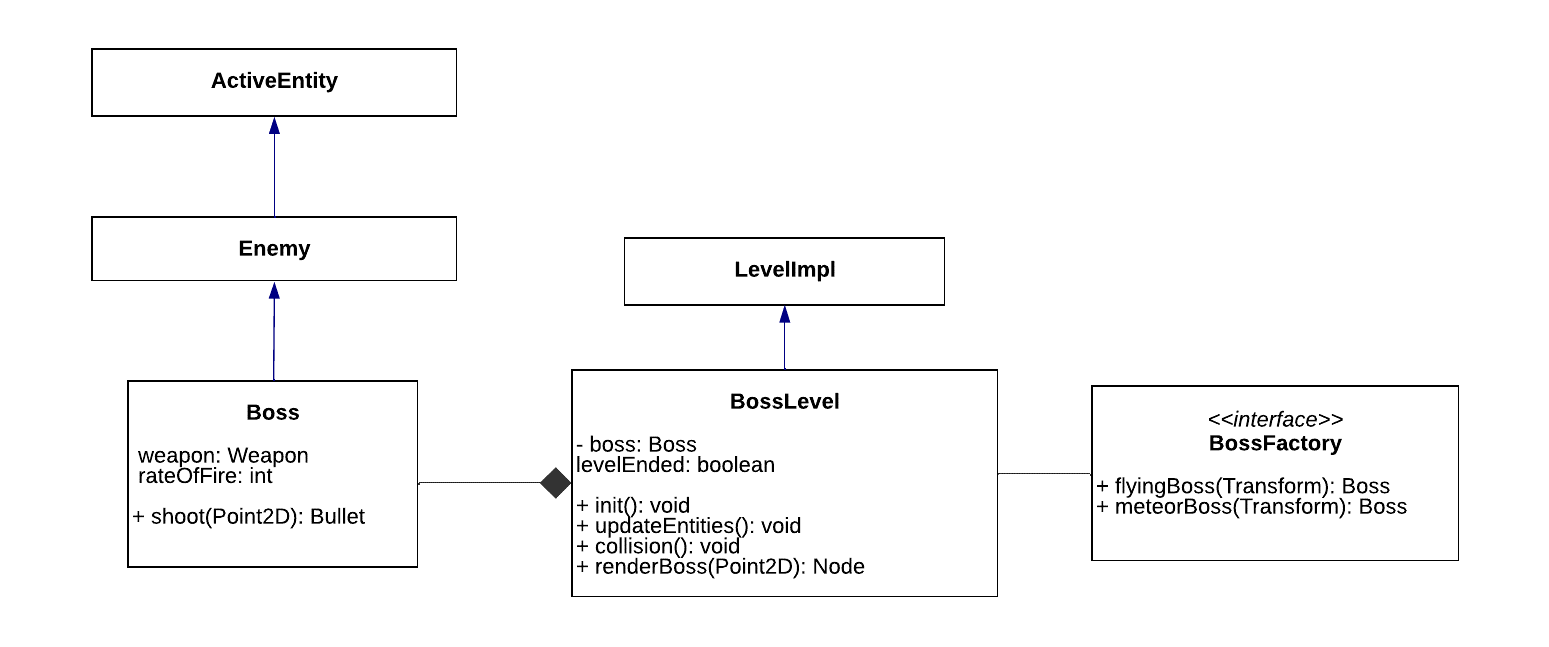
\includegraphics[width=1\textwidth]{UMLBoss.png}
    \caption{UML rappresentante le classi relative al Boss}
    \label{fig:schgen}
In fase di progettazione abbiamo deciso di implementare le boss fight in apposite stanze e quindi in particolari livelli BossLevel. All’interno di questi livelli sono gestiti tutti i component del Boss come Weapon e Transform.
Il Boss vero e proprio è generato da una factory che mi ha permesso di personalizzare i diversi Boss a livello di funzionamento specifico, implementandone, ad esempio, uno capace di volare.
La classe Boss, estendendo Enemy, possiede tutti i suoi component e è capace di seguire dei Behaviour se inizializzati. Ciò che lo differenzia da un generico Enemy, oltre alla difficoltà incontrata nel combatterlo, è la presenza del component Weapon, che gli permettere di sparare.
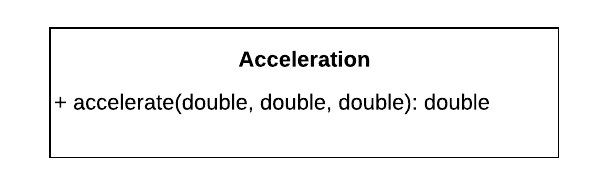
\includegraphics[width=1\textwidth]{UMLAcceleration.png}
    \caption{La classe Acceleration}
    \label{fig:schgen}
Infine ho implementato la classe di util Acceleration utilizzata nel movimento delle Entity per creare un effetto di movimento più fluido possibile.
\section{Sviluppo}
\subsection{Testing automatizzato}
Sono state realizzate due classi di test, per valutare l'effettiva efficienza del gioco, implementate attraverso la libreria JUnit:
\begin{itemize}
    \item TestEntity: controllo collisioni e danno
    \item TestFinalGrade: controllo del corretto calcolo del punteggio finale
\end{itemize}
\subsection{Metodologie di lavoro}
Abbiamo iniziato lo sviluppo vero e proprio del software basandoci sulla fase di progettazione del design architetturale precedentemente effettuata. Inizialmente avevamo pensato ad una gerarchia di entità più articolata, rendendoci poi conto che questa contrastava con i principi del pattern architetturale da noi scelto; di conseguenza abbiamo dovuto effettuare delle modifiche in fase di integrazione, adeguando il design di partenza.
Per approcciarci alla realizzazione di questo progetto, abbiamo utilizzato il DVCS Git che ci ha permesso di coordinarne agevolmente lo sviluppo, integrando le varie parti con facilità. Abbiamo scelto di adottare una metodologia ispirata a GitFlow: il nostro branch principale è il 'master', nel quale abbiamo committato la versione corretta e funzionante del gioco; il branch di sviluppo di default è il 'develop' abbiamo creato inoltre dei branch dedicati allo sviluppo di particolari feature del gioco. 
Vista la portata di lavoro del progetto, che nessuno di noi aveva mai affrontato in precedenza, abbiamo favorito il lavoro di gruppo e il confronto per la risoluzione dei problemi che si sono presentati.
\subsection{Note di sviluppo}
\subsubsection{Livia Cardaccia}
\small
\textbf{Utilizzo della libreria JavaFX}
\newline
Utilizzata per l'implementazione del menu di gioco. Un esempio è https://github.com/dennnanni/
UNIBOssfight/blob/master/UNIBOSSfight/src/main/java/app/ui/ViewManager.java
\newline
\textbf{Utilizzo di lambda expressions}
\newline
Utilizzate in più punti del codice. Un esempio è la classe https://github.com/dennnanni/
UNIBOssfight/blob/master/UNIBOSSfight/src/main/java/app/impl/builder/BehaviourBuilderImpl.java
\newline 
\textbf{Uso di Optional}
\newline
Utilizzati come tipo di ritorno dei metodi della classe \texttt{BehaviourImpl} https://github.com/dennnanni/
UNIBOssfight/blob/master/UNIBOSSfight/src/main/java/app/impl/component/BehaviourImpl.java
\newline
\textbf{Programmazione funzionale}
\newline
\texttt{Biconsumer} e \texttt{Bifunction} utilizzati nell'implementazione del component Behaviour. Di seguito l'interfaccia https://github.com/dennnanni/
UNIBOssfight/blob/master/UNIBOSSfight/
src/main/java/app/core/component/Behaviour.java
\newline 
\newline
\large
Per capire il funzionamento della libreria JavaFX mi sono inizialmente affidata alla documentazione online; alcune parti di codice del menu di gioco, in particolare quelle relative alla creazione dei bottoni e l'implementazione dei listeners per ognuno di essi, sono riadattate da codice del seguente progetto https://github.com/smowgli/space-runner-game-javafx/blob/main/src/model/SpaceRunnerButton.java
\subsubsection{Denise Nanni}
\small
\textbf{Utilizzo di lambda expressions}
\newline
Utilizzate per valorizzare i comportamenti alla collisione. Un esempio è https://github.com/dennnanni/
UNIBOssfight/blob/master/UNIBOSSfight/
src/main/java/app/impl/entity/EnemyImpl.java
\newline
\textbf{Utilizzo di Stream}
\newline
Utilizzati in questa classe https://github.com/dennnanni/
UNIBOssfight/blob/master/UNIBOSSfight/
src/main/java/app/game/Score.java
\subsubsection{Giovanni Prete}
\subsubsection{Matteo Sartini}
\textbf{Utilizzo di lambda expressions}
\newline
Utilizzate nel metodo addFlying() della classe BehaviourBuilderImpl per l'implementazione di un Behaviour per permettere al Boss di volare.
https://github.com/dennnanni/
UNIBOssfight/blob/master/UNIBOSSfight/
src/main/java/app/impl/builder/BehaviourBuilderImpl.java
\textbf{Utilizzo di Stream}
\newline
Utilizzati nella classe BossLevel per la gestione delle collisioni del Boss.
https://github.com/dennnanni/
UNIBOssfight/blob/master/UNIBOSSfight/
src/main/java/app/impl/level/BossLevel.java

Inoltre per implementare le classe di utilità con più contenuto matematico ho utilizzato una serie di tutorial matematici della serie “Math for game developers” del canale YouTube “Jorge Rodriguez” che è possibile consultare al seguente link:
https://www.youtube.com/playlist?list=PLW3Zl3wyJwWOpdhYedlD-yCB7WQoHf-My
\large
\section{Commenti finali}
\subsection{Autovalutazione e lavori futuri}
\subsubsection{Livia Cardaccia}
Dall'inizio del mio percorso universitario, questo è stato senza dubbio il lavoro più impegnativo: ha richiesto tempo e concentrazione ma soprattutto conoscenze che non avevo ancora completamente sviluppato durante il corso in aula ma che ho avuto l'occasione di approfondire durante la realizzazione del progetto. Lavorare in gruppo è stato un punto di forza, ci siamo confrontati e consigliati, il supporto che ci siamo dati l'un l'altro è stato secondo me fondamentale per la buona riuscita del progetto. Una delle difficoltà più grandi che ho incontrato è stata scrivere codice pulito e soprattutto efficiente ma anche trovare soluzioni efficaci per i problemi presentatisi in itinere, affrontandoli riflettendo e analizzando le possibili soluzioni. Credo che questo percorso abbia permesso di migliorarmi sotto questi aspetti e che possa essere uno slancio per continuare a perfezionare le mie capacità. 
\subsubsection{Denise Nanni}
\subsubsection{Giovanni Prete}
\subsubsection{Matteo Sartini}
Nonostante le numerose difficoltà incontrate durante lo sviluppo, trovo che l’applicativo che ne è nato sia, con le sue numerose imperfezioni dovute alla poca esperienza del gruppo e alla complessità del progetto visualizzato in fase di progettazione, un prodotto abbastanza completo e per il quale mi ritengo molto soddisfatto.
Trovo però che la parte più stimolante del progetto sia stato il teamwork necessario al suo completamento. Ritengo infatti che la collaborazione tra i vari componenti di un team sia una skill assolutamente indispensabile nel nostro campo lavorativo, e troppo spesso ignorata in contesti scolastici.
\subsection{Difficoltà incontrate e commenti per i docenti}
\section{Guida utente}
All'avvio del gioco si apre una schermata con il menu principale, in cui troviamo: un pulsante "play" per iniziare una nuova partita, un pulsante "level" per scegliere uno fra i due livelli proposti, un pulsante "help" per una breve spiegazione della modalità di gioco e un pulsante "score". 
Cliccando quest'ultimo si possono visualizzare le proprie statistiche di gioco e una voce "final grade" che assegna al giocatore un punteggio in base alle sue prestazioni, nell'ottica del conseguimento della laurea.
Avviata una partita, per giocare è necessario: premere il tasto 'd' per correre in avanti, premere il tasto 'a' per correre indietro, usare la barra spaziatrice per saltare e il puntatore del mouse per mirare ai nemici, a cui si spara cliccando.
Terminata una partita vi è la possibilità di tornare alla home con un apposito pulsante o proseguire con il gioco.
\section{Esercitazioni di laboratorio}
\subsection{livia.cardaccia@studio.unibo.it}
\begin{itemize}
    \item Laboratorio 03: https://virtuale.unibo.it/mod/forum/discuss
    .php?d=112846\#p168413
    \item Laboratorio 05: https://virtuale.unibo.it/mod/forum/discuss
    .php?d=114647\#p169868
    \item Laboratorio 06: https://virtuale.unibo.it/mod/forum/discuss
    .php?d=115548\#p172236
    \item Laboratorio 07: https://virtuale.unibo.it/mod/forum/discuss
    .php?d=117044\#p173315
    \item Laboratorio 08: https://virtuale.unibo.it/mod/forum/discuss
    .php?d=117852\#p174528
    \item Laboratorio 09: https://virtuale.unibo.it/mod/forum/discuss
    .php?d=118995\#p175251
    \item Laboratorio 10:
    https://virtuale.unibo.it/mod/forum/discuss
    .php?d=119938\#p176896
    \item Laboratorio 11: https://virtuale.unibo.it/mod/forum/discuss
    .php?d=121130\#p177745  
\end{itemize}
\subsection{denise.nanni@studio.unibo.it}
\begin{itemize}
    \item Laboratorio 06: https://virtuale.unibo.it/mod/forum/discuss
    .php?d=115548\#p171388
    \item Laboratorio 07: https://virtuale.unibo.it/mod/forum/discuss
    .php?d=117044\#p173321
    \item Laboratorio 09: https://virtuale.unibo.it/mod/forum/discuss
    .php?d=118995\#p175210
    \item Laboratorio 10: https://virtuale.unibo.it/mod/forum/discuss
    .php?d=119938\#p176543
\end{itemize}


\end{document}
